\documentclass[10pt]{article}\usepackage[nu]{esial}
\CSH\sloppy
\usepackage[utf8]{inputenc}
\usepackage{url}
\usepackage{geometry}
\usepackage{fancybox,moreverb}

\newcommand{\cd}[1]{\medskip\noindent\file{\null\hspace{-1em}[#1] }}
\newcommand{\touche}[1]{\hbox{$<$#1$>$}}
\newcommand{\ctrl}[1]{\touche{ctrl-#1}}
\newcommand{\tab}{\touche{TAB}}
%\hypersetup{colorlinks=false,pdfborder={0 0 0}}

\begin{document}
\title{TD2: Encore des pointeurs\ldots}
\maketitle

\bigskip\bigskip\Exercice Un programme C contient la déclaration suivante\,:

\medskip

\begin{boxedverbatim}
  char *couleur[6] = {"rouge", "vert", "bleu", "blanc", "noir","jaune"};
\end{boxedverbatim}

\Question Que représente {\tt couleur}\,?

\begin{Reponse}
  C'est un tableau de 6 pointeurs vers des chaines de caractères. Un
  schéma au tableau permet de mieux expliquer cela et ce qui suit
  \ldots
\end{Reponse}

\Question Que  désigne {\tt couleur + 2}\,?

\Question Quelle est la valeur de {\tt *couleur}\,?

\Question Quelle est la valeur de {\tt *couleur + 2}\,?

\begin{Reponse}
\begin{verbatim} 
    couleur + 2 = &couleur[2] et *(couleur+2)=couleur[2]=''bleu''
    *couleur = couleur [0] = ``rouge''
    *couleur+2 = ``uge''
\end{verbatim}

\noindent\verb?*couleur? pointe sur le premier élément de la chaine ``rouge''
soit 'r'. Si on rajoute 2 ($= 2 \times sizeof(char)$), ça pointera sur 'u'. La
fin de la chaine est après 'e' de ``rouge''.
\end{Reponse}

\Question Quelle est la valeur de {\tt *(*(couleur + 5) +3)}\,? (Même
question avec +4, +5, +6).

\begin{Reponse}
\begin{verbatim} 
   *(*(couleur + 5) +3) = 'n' 
   En effet : 
     *(couleur + 5) = ``jaune'' , ``jaune'' étant situé à couleur[5] 
     *(couleur + 5) +3 = ``ne''

   *(*(couleur + 5) +4) = 'e' 
   *(*(couleur + 5) +5) = '\0' 
   *(*(couleur + 5) +6) = 'c' , c quelconque 
\end{verbatim}
~
\end{Reponse}




\bigskip\bigskip\Exercice {\bf Pointeurs et structures.}
%----------------------------------------

Soit le type suivant\,:


\medskip

\begin{boxedverbatim}
  typedef struct {
    char nomPlanete[MAX_CAR];
    int  rayon;  
  } Planete;
\end{boxedverbatim}


\Question Quelle est l'instruction qui permet de créer une variable
{\em pointeur sur Planete}\,?

\begin{Reponse}
  \begin{boxedverbatim} 
    Planete *p1;
    p1 = (Planete *) malloc (sizeof(Planete));
  \end{boxedverbatim}
~
\end{Reponse}
	  
\Question Ecrire une fonction qui saisit les données relatives à une
planète.

\begin{Reponse}
  \begin{boxedverbatim} 
    void Saisir(Planete *p){
  
      printf("Donner nom planète : ");
      scanf ("%s",p->nomPlanete);
      printf("Donner son rayon : ");
      scanf ("%d",&p->rayon);
    } 
  \end{boxedverbatim}
~
\end{Reponse}

\Question Ecrire une fonction qui duplique une planète. 

\begin{Reponse}
  \begin{boxedverbatim} 
    Planete* Dupliquer(Planete p){
  
      Planete *p1;
      p1 = (Planete *) malloc (sizeof(Planete));
      
      strcpy(p1->nomPlanete, p.nomPlanete);
      p1->rayon = p.rayon;
      
      return (p1);
    }
    
  \end{boxedverbatim}
~
\end{Reponse}

\Question  Soit l'extrait suivant permettant de tester les fonctions
précédentes\,;


\medskip


\begin{boxedverbatim}
void main()
{
  Planete p;
  Planete *ptr_p;
  Saisir(&p);
  printf("%s %d \n", p.nomPlanete, p.rayon);
  ptr_p = Dupliquer(p);
  printf("%s %d \n", ptr_p->nomPlanete, ptr_p->rayon);
}
\end{boxedverbatim}


\bigskip Comment s'analysent les types des différentes références
suivantes\,:

\bigskip

\begin{tabular}{|p{.2\linewidth}|p{.3\linewidth}|}
  \hline
  Référence  &             Type         \\\hline
  \verb+ptr_p+     &               \\\hline                  
  \verb+*ptr_p+         &         \\\hline            
  \verb+ptr_p->nomPlanete+& \\\hline
  \verb+ptr_p->rayon+& \\\hline
  \verb+p+& \\\hline
  \verb+&p+& \\\hline
  \verb+p.nomPlanete+& \\\hline
  \verb+p.rayon+& \\\hline
\end{tabular}


\begin{Reponse}

\begin{tabular}{|p{.2\linewidth}|p{.3\linewidth}|}
  \hline
  Référence  &             Type         \\\hline
  \verb+ptr_p+     &      Planete *         \\\hline                  
  \verb+*ptr_p+         &  Planete       \\\hline            
  \verb+ptr_p->nomPlanete+& char []\\\hline
  \verb+ptr_p->rayon+& int\\\hline
  \verb+p+& Planete\\\hline
  \verb+&p+& Planete*\\\hline
  \verb+p.nomPlanete+& char []\\\hline
  \verb+p.rayon+& int\\\hline
\end{tabular}
~
\end{Reponse}


 


\bigskip\bigskip\Exercice {\bf Chaînes de caractères.}
%--------------------------------------

\Question
Ecrire une fonction {\tt PremierCar(\ldots)} qui renvoie l'adresse de
la première occurence du 
caractère {\tt c} dans une chaîne de caractères dont l'adresse (du
premier caractère) est passé à l'argument {\tt ptrCar}\,:

\run{char *PremierCar(char c, char *ptrCar)}

\Question
Ecrire la fonction {\tt int main(int argc, char *argv[])} permettant
de tester la fonction. Un exemple d'exécution est\,:

\medskip

\begin{boxedverbatim}
./occurence  o Bonjour
\end{boxedverbatim}

\medskip

Le résultat affiché est le suivant\,:

\medskip

\begin{boxedverbatim}
La premiere occurence de 'o' dans 'Bonjour' est en position 1
\end{boxedverbatim}

\begin{Reponse}
  Cet exercice a été déjà fait en TP2 mais il y a une différence dans
  le type de retour qui est un pointeur au lieu d'un entier. Aussi, on
  fait usage des arguments en ligne de commande.

\begin{boxedverbatim}
#include <stdio.h>

char *PremierCar(char c, char *ptrCar){
  do
    if (*ptrCar == c)
      return (ptrCar);
  while (*ptrCar++);

  return (NULL);
}

int main(int argc, char * argv[]){

  char c, *str, *adrPremCar;

  c = argv[1][0]; //argv[1] étant un pointeur vers une chaine de car.
                  // argv[1][0] est le premier car de cette chaine
  str = argv[2];

  if ( (adrPremCar = PremierCar(c,str)) == NULL) 
    printf ("'%c' n'est pas dans %s.\n",c,str);
  else
    printf ("La premiere occurence de '%c' dans %s est en position
    %d.\n", c,str,adrPremCar - str);
}
\end{boxedverbatim}
\end{Reponse}
    



\bigskip\bigskip\Exercice {\bf Filiation.}
%--------------------------------

Sous Unix, il existe un ensemble de pointeurs représentant la
filiation des  processus\,: 

Dans la figure \ref{filiation}, {\tt fils A} est le premier processus
fils créé par le processus père, {\tt fils B} est le deuxième fils
créé par le processus père \ldots etc.
Chaque fils peut évidemment créer des fils, et le père est également le
fils d'un autre processus.

Nous supposons pour simplifier que chaque processus est caractérisé
par un numéro (entier positif).
%Il n'existe qu'une seule filiation par machine, tous les processus
%appartiennent donc à cette unique filiation.


\bigskip\bigskip
\begin{figure}[h]
  \centerline{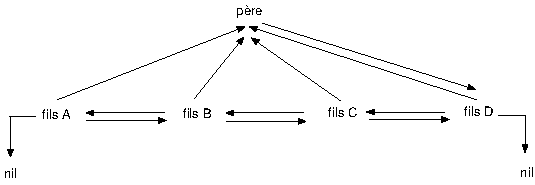
\includegraphics[width=\linewidth]{filiation.pdf}}
  \caption[]
	  {{\it Filiation sous Unix}}
	  \label{filiation}
\end{figure}
\bigskip

\Question  Représenter schématiquement, sous la
forme d'une structure de données, un n\oe ud (c'est à dire un
processus) de cette filiation, puis écrire la définition de cette
structure en langage C.

\Question  Le processus repéré par la variable
pointeur {\tt p} vient de créer un processus fils de numéro {\tt no}.
Ecrire en langage C la fonction {\tt maj} qui met à jour la filiation
des processus.

\begin{Reponse}
\vspace{-.7cm}
\begin{verbatim}
struct proc{
  unsigned int noproc;
  struct proc *pere, *frere_g, *frere_d, *dernier_fils;
  
};

void maj(struct proc *p, int no){
  struct proc *fils;
  fils = (struct proc *) malloc ((unsigned int)(sizeof(struct proc)));

  fils->noproc = no;
  fils->pere = p;
  fils->frere_d = NULL;
  fils->dernier_fils = NULL 

  if (p->dernier_fils != NULL){
    //le père a déjà des fils, le dernier fils devient le frère à
    //gauche et aura un frère à sa droite
    fils->frere_g = p->dernier_fils;
    p->dernier_fils->frere_d = fils;
  } else {// le père n'avait pas de fils
    fils->frere_g = NULL;
    p->dernier_fils = fils;
  } 
}
\end{verbatim}
~
\end{Reponse}



\end{document}

%%% Local Variables:
%%% coding: utf-8
